% !TeX root = ../main.tex
\chapter{机器学习}

从历史上看,\keyterm{深度学习}属于更广泛的统计\keyterm{机器学习}领域,因为从本质上它关注从数据中学习表示的方法。其所涉及的技术最初来自\keyterm{人工神经网络},``深度''一词强调模型是长映射组合,目前已经验证可以获得更好的表现。

深度模型的模块化、多功能性和可扩展性催生了大量特定的数学方法和软件开发工具,使深度学习成为一个独特而广阔的技术领域。

\section{从数据中学习}\label{sec1.1}

从数据训练模型最简单的用例是当信号 $x$ 输入时,例如车牌图片,人们想要从中预测量 $y$,例如车牌上的字符串。

在许多现实世界场景中,$x$ 是在不受控制的环境中捕获的高维信号,因此给出将 $x$ 和 $y$ 相关联的分析方法十分复杂。

我们能做的就是收集一个由 $(x_n, y_n)$ 对组成的大型\keyterm{训练集} $\mathcal{D}$,并设计一个\keyterm{参数模型} $f$。它是一段计算机代码,其中包含可调节其行为的\keyterm{可训练参数} $w$,因此,使用适当的 $w^*$ 值,就会得到一个良好的预测器。这里的``良好''意味着如果将 $x$ 输入这段代码,则它计算的值 $\hat{y}= f(x;w^*)$ 是对 $y$ 的良好估计,如果有的话,该估计与训练集中的 $x$ 相关联。

这里``良好''的概念通常用\keyterm{损失} $\mathcal{L}(w)$ 来形式化,当 $f(\cdot;w)$ 在 $\mathcal{D}$ 上表现良好时,损失会很小。然后,\keyterm{训练}模型就是计算使 $\mathcal{L}(w^*)$ 最小的 $w^*$ 值。本书的大部分内容都是关于 $f$ 的定义,在现实场景中,$f$ 是预先定义子模块的复杂组合。

组成 $w$ 的可训练参数通常称为\keyterm{权重},类似于生物神经网络的突触权重。除了这些参数之外,模型通常还依赖于\keyterm{元参数},这些元参数是根据领域先验知识、最佳实践或资源限制设置的。它们也可以以某种方式进行优化,但使用的技术不同于用于优化 $w$ 的技术。

\section{基函数回归}\label{sec1.2}

我们通过一个简单的例子来说明模型的训练,其中 $x_n$ 和 $y_n$ 为两个实数,损失为\keyterm{均方误差}:
\begin{equation}
    \mathcal{L}(w) = \frac{1}{N}\sum_{n=1}^{N}\big(y_n-f(x_n;w)\big)^2\label{eq1.1}
\end{equation}
$f(\cdot;w)$ 是预定义基函数 $f_1, \dots , f_K$ 的线性组合,其中 $w =(w_1, \dots ,w_K)$:
\[f(x;w) = \sum_{k=1}^{K}w_kf_k(x)\]
\begin{figure}
    \centering
    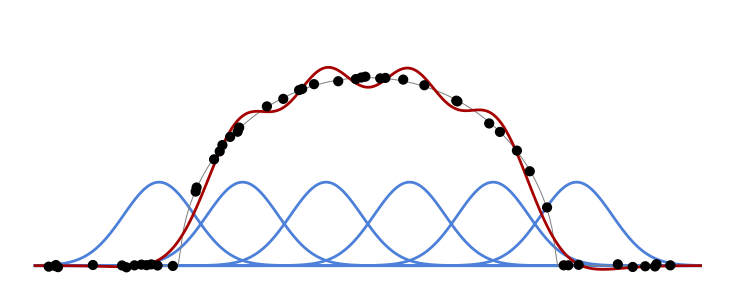
\includegraphics[width=0.9\textwidth]{fig/fig1.1.png}
    \caption[核回归]{给定基函数基础(蓝色曲线)和训练集(黑点),我们可以计算前者的最佳线性组合(红色曲线),以近似后者的均方误差。}
    \label{fig1.1}
\end{figure}
由于 $f(x_n;w)$ 相对于 $w_k$ 是线性的,并且 $\mathcal{L}(w)$ 相对于 $f(x_n;w)$ 是二次的,因此损失 $\mathcal{L}(w)$ 相对于 $w_k$ 是二次的,$w^*$ 最小化损失归结为求解线性系统。请参阅图 \ref{fig1.1} 中以高斯核为 $f_k$ 的示例。

\section{欠拟合和过拟合}

一个关键要素是模型\keyterm{能力}与训练数据之间的相互作用,即模型的灵活性和适应不同数据的能力与训练数据的数量和质量之间的相互作用。当能力不足时,模型无法拟合数据,导致训练时误差较高。这被称为\keyterm{欠拟合}。

相反,当数据量不足时,如图 \ref{fig1.2} 所示,模型通常会学到特定于训练样本的特征,从而在训练过程中获得优异的表现,
\begin{figure}
    \centering
    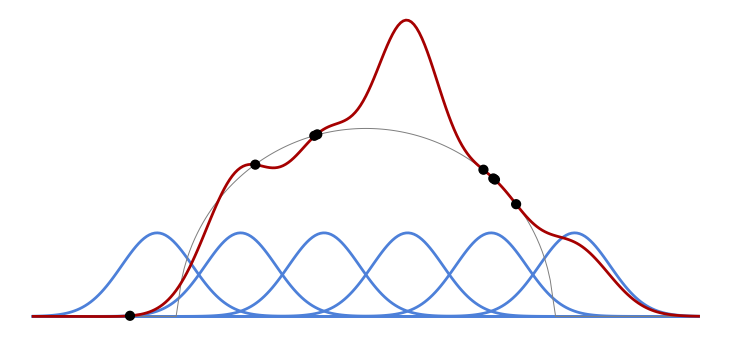
\includegraphics[width=0.9\textwidth]{fig/fig1.2.png}
    \caption[核回归的过拟合]{如果训练数据量(黑点)与模型能力相比较小,则训练期间拟合模型的经验表现(红色曲线)反映出对底层数据结构(细黑色曲线)的实际拟合很差,因此其预测的有效性不佳。}
    \label{fig1.2}
\end{figure}
但代价是与数据的全局结构拟合较差,并且在新输入上表现不佳。这种现象称为\keyterm{过拟合}。

因此,应用\keyterm{机器学习}艺术很大一部分在于设计不太灵活但仍然能够适应数据的模型。这是通过在模型中设计正确的\keyterm{归纳偏置}来实现的,这意味着其结构对应于手头数据的底层结构。

尽管这种经典观点与合理大小的深度模型相关,而对于具有大量可训练参数和极端能力但在预测方面仍表现良好的大型模型来说,事情会变得混乱。我们将在 \ref{sec3.6} 节和 \ref{sec3.7} 节再次讨论这一点。

\section{模型分类}

我们可以将\keyterm{机器学习}模型的使用分为三类:

\begin{itemize}
    \item \keyterm{回归}包括预测一个连续值向量 $y \in \mathbb{R}^K$,例如,给定一个输入信号 $X$,预测一个物体的几何位置。这是我们在 \ref{sec1.2} 节所学内容的多维泛化。训练集由一对输入信号和\keyterm{基本事实}值组成。
    \item \keyterm{分类}旨在是从有限集合 ${1,\dots,C}$ 中预测值,例如,预测图像 $X$ 的标签 $Y$。与回归一样,训练集由一对输入信号和基本事实量组成,基本事实量在这里是该集合中的一个标签。解决这个问题的标准方法是为每个潜在类别预测一个分数,使得正确的类别具有最高分数。
    \item \keyterm{密度建模}的目标是对数据 $\mu X$ 本身(例如图像)的概率密度函数进行建模。在这种情况下,训练集由值 $x_n$ 组成,没有要预测的关联量,并且训练后的模型能够评估概率密度函数,或从分布中采样,或两者兼而有之。
\end{itemize}

回归和分类通常被称为\keyterm{监督学习},因为必须提供在训练过程中需要预测的值,例如由人类专家提供。相反,密度建模通常被视为\keyterm{无监督学习},因为它只需要使用现有数据而无需生成相关的基本事实。

这三个类别并不是互不相干的;例如,分类可以被转换为类别分数回归,或者离散序列密度建模可以被看作迭代分类。此外,它们并不涵盖所有情况。有时我们可能希望预测复合量,或者多个类别,或者在信号条件下对密度进行建模。